\documentclass{article}
\usepackage[T1]{fontenc}
\usepackage[utf8]{inputenc}
\usepackage{lmodern}
\usepackage[polish,shorthands=off]{babel}
\usepackage{graphicx}
\usepackage{fancyhdr}
\pagestyle{fancy}
\lhead{}
\chead{Sprawozdanie z Laboratorium 1 \\ Obliczenia Naukowe}
\rhead{}
\rfoot{Jakub Kowal}

\title{Sprawozdanie z Laboratorium 1 \\ Obliczenia Naukowe}
\author{Jakub Kowal}
\begin{document}
\section{Zadanie 1}
Opis problemu:
W zadaniu należało wyznaczyć następujące wartości:
\begin{itemize}
        % \item $pc_{32}$ - suma iloczynów odpowiadających sobie
    \item $Macheps$ --- najmniejsza liczba $\mathrm{macheps}>0$ taka, że $\mathrm{fl}(1.0+\mathrm{macheps})>1.0$ i $\mathrm{fl}(1.0+\mathrm{macheps})=1+\mathrm{macheps}$
    \item $eta$ --- najmniejsza dodatnia liczba zmiennoprzecinkowa (najmniejsza liczba nieznormalizowana --- $\mathrm{MIN}_{\mathrm{sub}}$)
    \item liczba $MAX$ --- największa liczba nieznormalizowana --- $\mathrm{MAX}_{\mathrm{sub}}$
\end{itemize}
Oraz odpowiedzieć na pytania:
\begin{itemize}
    \item Jaki związek ma liczba $macheps$ z $precyzją$ $arytmetyki$ (oznaczaną na wykładzie przez $\epsilon$)?
    \item Jaki związek ma liczba $eta$ z liczbą $\mathrm{MIN}_{\mathrm{sub}}$?
    \item Co zwracają funkcje floatmin(Float32) i floatmin(Float64) i jaki jest związek zwracanych wartości z liczbą $\mathrm{MIN}_{\mathrm{nor}}$?
\end{itemize}
Wyniki:
\subsection{$Macheps$}
\subsubsection{Float64}
eps(Float64) = 2.220446049250313e-16 \newline
Mój wynik: 2.220446049250313e-16 \newline
\subsubsection{Float32}
eps(Float32) = 1.1920929e-07 \newline
Mój wynik: 1.1920929e-07 \newline
\subsubsection{Float16}
eps(Float16) = 0.000977 \newline
Mój wynik: 0.0009765625 \newline
\subsection{$eta$}
\subsubsection{Float64}
nextfloat(Float64(0.0)) = 5.0e-324 \newline
Mój wynik: 5.0e-324
\subsubsection{Float32}
nextfloat(Float32(0.0)) = 1.0e-45 \newline
Mój wynik: 1.0e-45
\subsubsection{Float16}
nextfloat(Float16(0.0)) = 6.0e-8 \newline
Mój wynik: 6.0e-8
\subsection{$MAX$}
\subsubsection{Float64}
floatmax(Float64(0.0)) = 1.7976931348623157e308 \newline
Mój wynik: 1.7976931348623157e308 \newline
\subsubsection{Float32}
floatmax(Float32(0.0)) = 3.4028235e38 \newline
Mój wynik: 3.4028235e38 \newline
\subsubsection{Float16}
floatmax(Float16(0.0)) = 6.55e4 \newline
Mój wynik: 6.55e4 \newline
\subsection{Wartości z float.h:}
\subsubsection{FLOAT}
FLT\_MAX = 3.4028234664e+38 \newline
FLT\_MIN = 1.1754943508e-38 \newline
FLT\_EPSILON = 1.1920928955e-07 \newline
\subsubsection{DOUBLE}
DBL\_MAX = 1.79769313486231570815e+308\newline
DBL\_MIN = 2.22507385850720138309e-308\newline
DBL\_EPSILON = 2.22044604925031308085e-16\newline
\subsubsection{LONG DOUBLE}
LDBL\_MAX = 1.189731495357231765021263853031e+4932\newline
LDBL\_MIN = 3.362103143112093506262677817322e-4932\newline
LDBL\_EPSILON = 1.084202172485504434007452800870e-19\newline
\subsection{Odpowiedzi na pytania:}
\begin{enumerate}
\item Jaki związek ma liczba $macheps$ z $precyzją$ $arytmetyki$ (oznaczaną na wykładzie przez $\epsilon$)? \newline
Precyzja arytmetyki $ \epsilon = 0.5\beta^{1-t}$(macheps=$\beta^{1-t}$). Wynika to z tego, że błąd musi spełniać założenie $|\delta| \le \epsilon$ i $\mathrm{fl}(1.0+\delta) = 1.0$. Oznacza to, że nie może zostać zaokrąglony w górę, ponieważ wtedy będzie już następną liczbą.
    \item Jaki związek ma liczba $eta$ z liczbą $\mathrm{MIN}_{\mathrm{sub}}$?\newline
    $Min_{sub}=m_{min}*\beta ^{c_{min}}=\beta ^{1-t}*\beta ^{c_{min}}=\beta ^{c_{min}+(1-t)}$ \newline
    $MIN_{nor}=1*\beta ^{c_{min}}$\newline
    Liczba $eta$ = $Min_{sub}$
    \item Co zwracają funkcje floatmin(Float32) i floatmin(Float64) i jaki jest związek zwracanych wartości z liczbą $\mathrm{MIN}_{\mathrm{nor}}$?\newline
    Floatmin jest $MIN_{nor}$ dla danych typów
\end{enumerate}
\subsection{Wnioski}
Wyniki uzyskane w zadaniu są zgodne z wartościami podanymi w języku. Zauważamy, że eps() oznacza najmniejszą różnicę między liczbami w zakresie mantysy, a nextfloat() zwraca najmniejszą możliwą następną liczbę.
\section{Zadanie 2}
Opis problemu:
W zadanie trzeba było sprawdzić, czy wynik równania \newline $3(\frac{4}{3}-1)-1$ zwraca wartości epsilonu maszynowego\newline\newline
Wyniki:
\subsection{Float64}
eps(Float64) = 2.220446049250313e-16 \newline
Wynik równania: -2.220446049250313e-16 
\subsection{Float32}
eps(Float32) = 1.1920929e-07 \newline
Wynik równania: 1.1920929e-07
\subsection{Float16}
eps(Float16) = 0.000977 \newline
Wynik równania: -0.000977
\subsection{Wnioski}
Wyniki uzyskane w zadaniu są zgodne z wartościami eps() dla danych typów. Wynika to z faktu, że w obliczeniach występują błędy zaokrągleń, które powodują, że wynik jest równy eps() lub jego przeciwieństwu.
\section{Zadanie 3}
Opis problemu:
W zadaniu należało zbadać odległości między liczbami w arytmetyce zmiennoprzecinkowej w różnych przedziałach. Należało sprawdzić, czy liczba $2^{-52}$ jest taką odległością.\newline\newline
Wyniki:
\subsection{Przedział [1,2]}
$2^{-52}$ jest odległością między kolejnymi liczbami w tym przedziale. Możemy stwierdzić to na podstawie binarnego zapisu tych liczb. \newline
1: 0011111111110000000000000000000000000000000000000000000000000000 \newline
$2^{-52}$: 0011110010110000000000000000000000000000000000000000000000000000 \newline
1+$2^{-52}$: 0011111111110000000000000000000000000000000000000000000000000001 \newline
Różnią się one na ostatnim bicie, co oznacza, że $2^{-52}$ jest odległością między tymi liczbami.
\subsection{Przedział [2,4]}
W tym przedziale odległość między kolejnymi liczbami wynosi $2^{-51}$. Możemy stwierdzić to na podstawie binarnego zapisu tych liczb. \newline
2: 0100000000000000000000000000000000000000000000000000000000000000\newline
$2^{-52}$: 0011110010110000000000000000000000000000000000000000000000000000 \newline
2+$2^{-52}$: 0100000000000000000000000000000000000000000000000000000000000000 \newline
Jak widać dodanie $2^{-52}$ do liczby 2 nie zmienia jej wartości, co oznacza, że $2^{-52}$ mniejsze od odległości między tymi liczbami. Natomiast dodając $2^{-51}$ do liczby 2 otrzymujemy otrzymujemy następną liczbę w tym przedziale.
\subsection{Przedział [$\frac{1}{2}$,1]}
$\frac{1}{2}$: 0011111111100000000000000000000000000000000000000000000000000000 \newline
$2^{-52}$: 0011110010110000000000000000000000000000000000000000000000000000 \newline
$\frac{1}{2}$+$2^{-52}$: 0011111111100000000000000000000000000000000000000000000000000010 \newline
Różnią się one na przedostatnim bicie, co oznacza, że $2^{-52}$ jest dwukrotnie większa od odległości między tymi liczbami.
\subsection{Wnioski}
W zadaniu udało się potwierdzić, że odległości między liczbami w arytmetyce zmiennoprzecinkowej zależą od przedziału, w którym się znajdują. W przedziale [1,2] odległość ta wynosi $2^{-52}$, w przedziale [2,4] wynosi $2^{-51}$, a w przedziale [$\frac{1}{2}$,1] wynosi $2^{-53}$.
\section{Zadanie 4}
Opis problemu: \newline
W zadaniu należało znaleźć taką liczbę zmiennoprzecinkową $x \in (1,2)$, dla której $x*(\frac{1}{x}) \ne 1$. Należało również znaleźć najmniejszą taką liczbę.
\subsection{Wynik}
Liczba 1.000000057228997 jest najmniejsza liczbą spełniającą warunki zadania.
\subsection{Wnioski}
W x odległość między liczbami wynosi 2-52, ale w $\frac{1}{x}$ to już jest 2-53 (Ponieważ $\frac{1}{x} \in (\frac{1}{x},1)$). Wychodzi na to, że musi to być liczba, która przy dzieleniu jedynki zostanie zaokrąglona w górę oraz później przy mnożeniu przez siebie nie zostanie zaokrąglona w dół.
\section{Zadanie 5}
Opis problemu: \newline
W zadaniu należało zaimplementować funkcje obliczające iloczyn skalarny dwóch wektorów.\newline\newline
Wyniki:
\subsection{Float64}
\begin{enumerate}
    \renewcommand{\labelenumi}{\alph{enumi})}
    \item Wynik: 1.0251881368296672e-10
    \item Wynik: -1.5643308870494366e-10
    \item Wynik: 0.0
    \item Wynik: 0.0
\end{enumerate}
\subsection{Float32}
\begin{enumerate}
    \renewcommand{\labelenumi}{\alph{enumi})}
    \item Wynik: -0.4999443
    \item Wynik: -0.4543457
    \item Wynik: -0.5
    \item Wynik: -0.5
\end{enumerate}
\subsection{Wnioski}
W zadaniu nie udało się zbytnio zaobserwować wpływu redukcji liczb znaczących na wynik, ponieważ przypadki, gdzie dane były posortowane dały nam takie same wyniki. Zauważyć na pewno można jednak, że kolejność dodawania ma znaczenie, ponieważ dodawanie "od przodu" i "od tyłu" dały różne wyniki. Kierując się informacjami z wykładu wiemy, że redukcja cyfr znaczących występuje w momencie dodawania liczb skrajnie mniejszych do większych. Natomiast w przypadku odejmowania redukcja ta nachodzi przy liczbach bardzo do siebie zbliżonych.\newline
Poprawny wynik: $-1.00657107000000*10^{-11}$\newline
Najbliżej poprawnego wyniku była metoda b) dla Float64, czyli dodawanie "od tyłu".
\section{Zadanie 6}
Opis problemu: \newline
W zadniu należało zaimplementować dwie funkcje i porównać ich wyniki dla różnych wartości n.\newline
Funkcje:
\begin{itemize}
    \item $f(n) = \sqrt{x^{2}+1}-1$
    \item $g(n) = \frac{x^{2}}{\sqrt{x^{2}+1}+1}$
\end{itemize}
\subsection{Wyniki}
f(0.125)= 0.0077822185373186414\newline
g(0.125)= 0.0077822185373187065\newline
f(0.015625)= 0.00012206286282867573\newline
g(0.015625)= 0.00012206286282875901\newline
f(0.001953125)= 1.9073468138230965e-6\newline
g(0.001953125)= 1.907346813826566e-6\newline
f(0.000244140625)= 2.9802321943606103e-8\newline
g(0.000244140625)= 2.9802321943606116e-8\newline
f(3.0517578125e-5)= 4.656612873077393e-10\newline
g(3.0517578125e-5)= 4.6566128719931904e-10\newline
f(3.814697265625e-6)= 7.275957614183426e-12\newline
g(3.814697265625e-6)= 7.275957614156956e-12\newline
f(4.76837158203125e-7)= 1.1368683772161603e-13\newline
g(4.76837158203125e-7)= 1.1368683772160957e-13\newline
f(5.960464477539063e-8)= 1.7763568394002505e-15\newline
g(5.960464477539063e-8)= 1.7763568394002489e-15\newline
f(7.450580596923828e-9)= 0.0\newline
g(7.450580596923828e-9)= 2.7755575615628914e-17\newline
f(9.313225746154785e-10)= 0.0\newline
g(9.313225746154785e-10)= 4.336808689942018e-19\newline
\subsection{Wnioski}
Wyniki funkcji f i g są zbliżone dla większych wartości n, ale wraz ze zmniejszaniem się n, różnice między nimi rosną. Dla bardzo małych wartości n, funkcja f zwraca 0, podczas gdy funkcja g nadal zwraca wartości bliskie zeru, ale niezerowe. Wynika to z faktu, że w odejmowaniu w funkcji f następuje redukacja cufr znaczących. Wynika to z faktu, że $\sqrt{x^{2}+1}$ wraz ze wzrostem x zbliża się do 1, co powoduje, że różnica między nimi staje się bardzo mała i prowadzi do utraty precyzji.
\section{Zadanie 7}
Opis problemu: \newline
W zadaniu należało zaimplementować funkcję obliczającą wartość pochodnej funkcji $f(x) = \sin(x) + \cos(3x)$ w punkcie $x_{0} = 1$ za pomocą wzoru $f`(x_{0}) = \frac{f(x_{0}+h)-f(x_{0})}{h}$ oraz wzory pochodnej $f`(x)=\cos(x)-3\sin(3x)$
\subsection{Wyniki}
\begin{figure}[ht!]
\centering
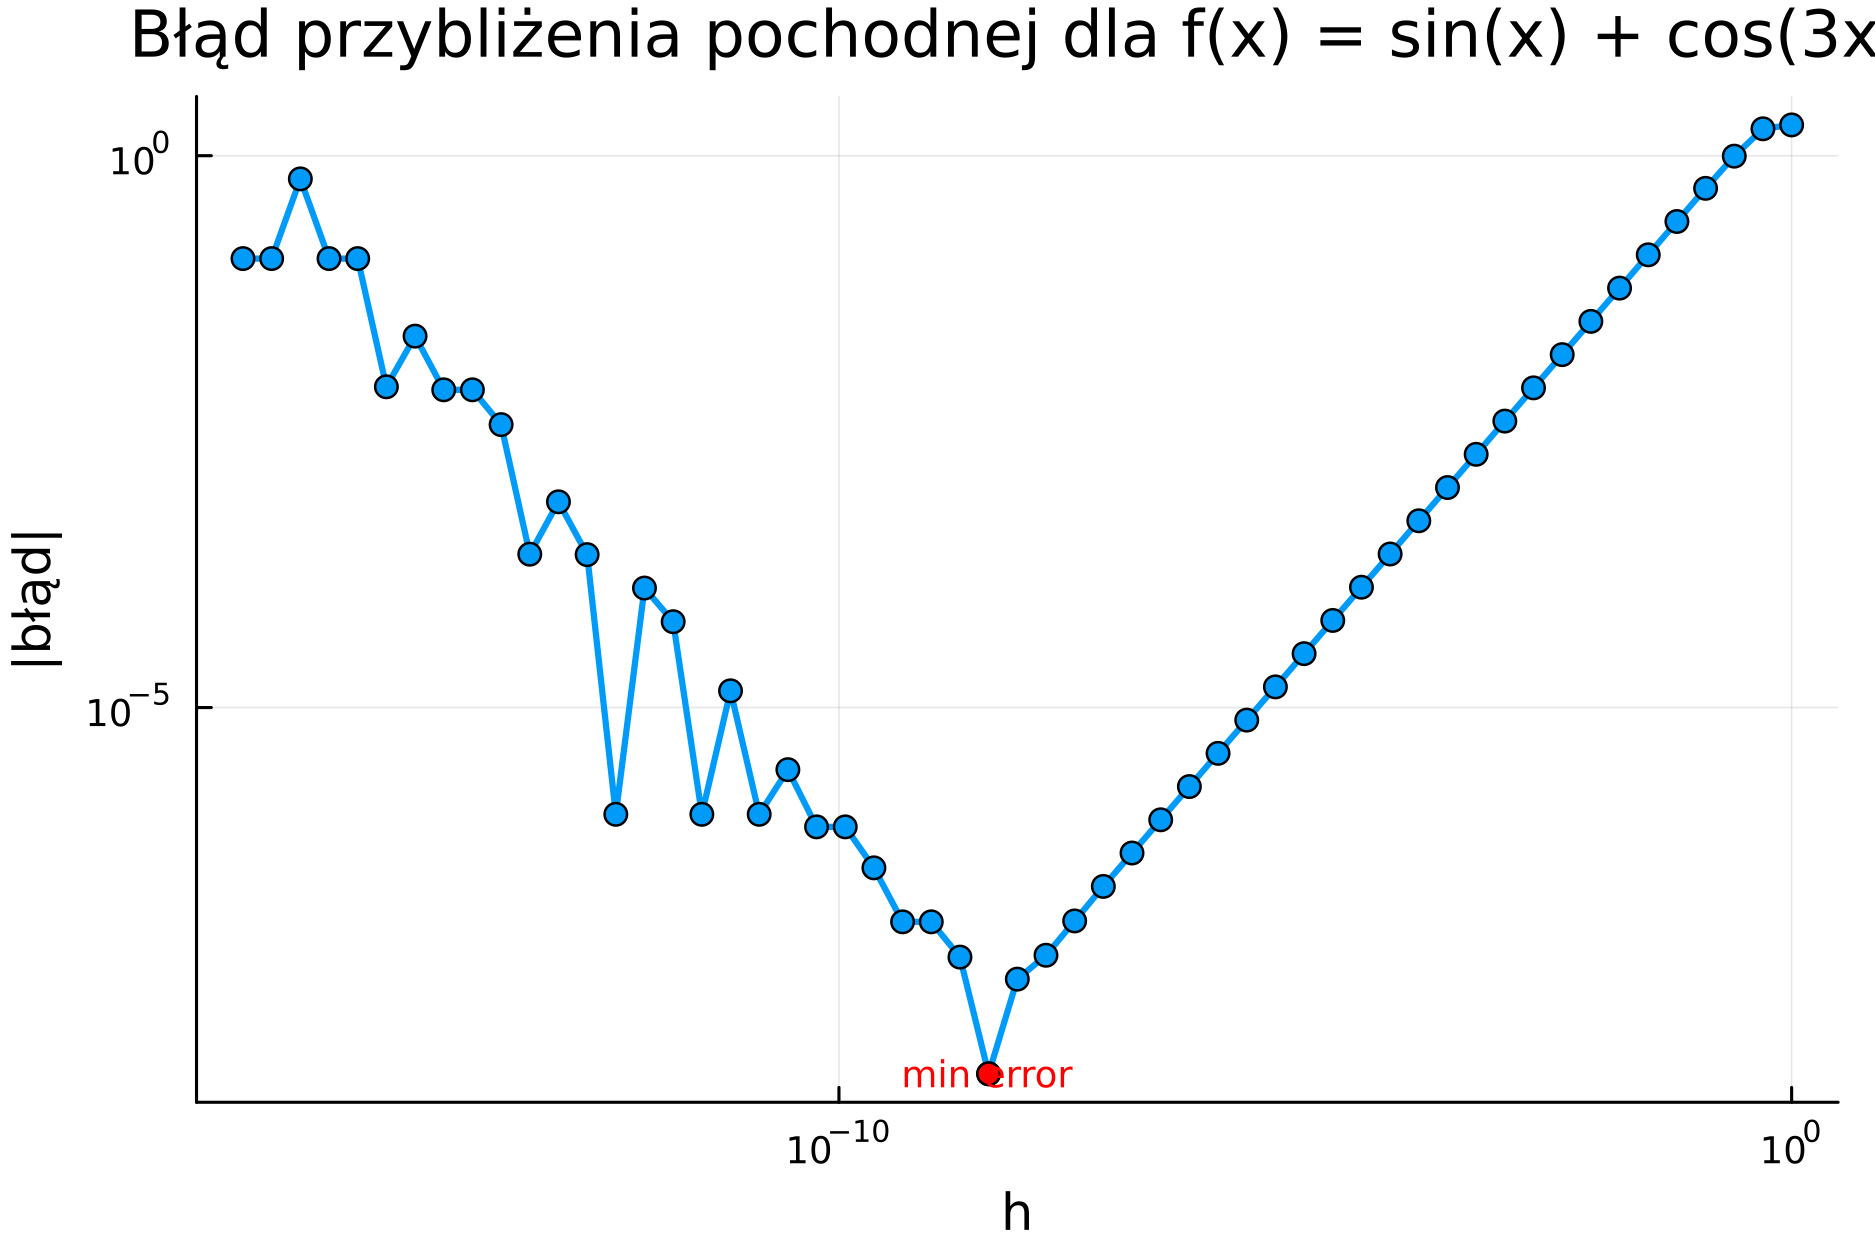
\includegraphics[width=97mm]{plot_1.jpg}
\caption{Błąd przybliżenia pochodnej}
\end{figure}
\begin{figure}[ht!]
\centering
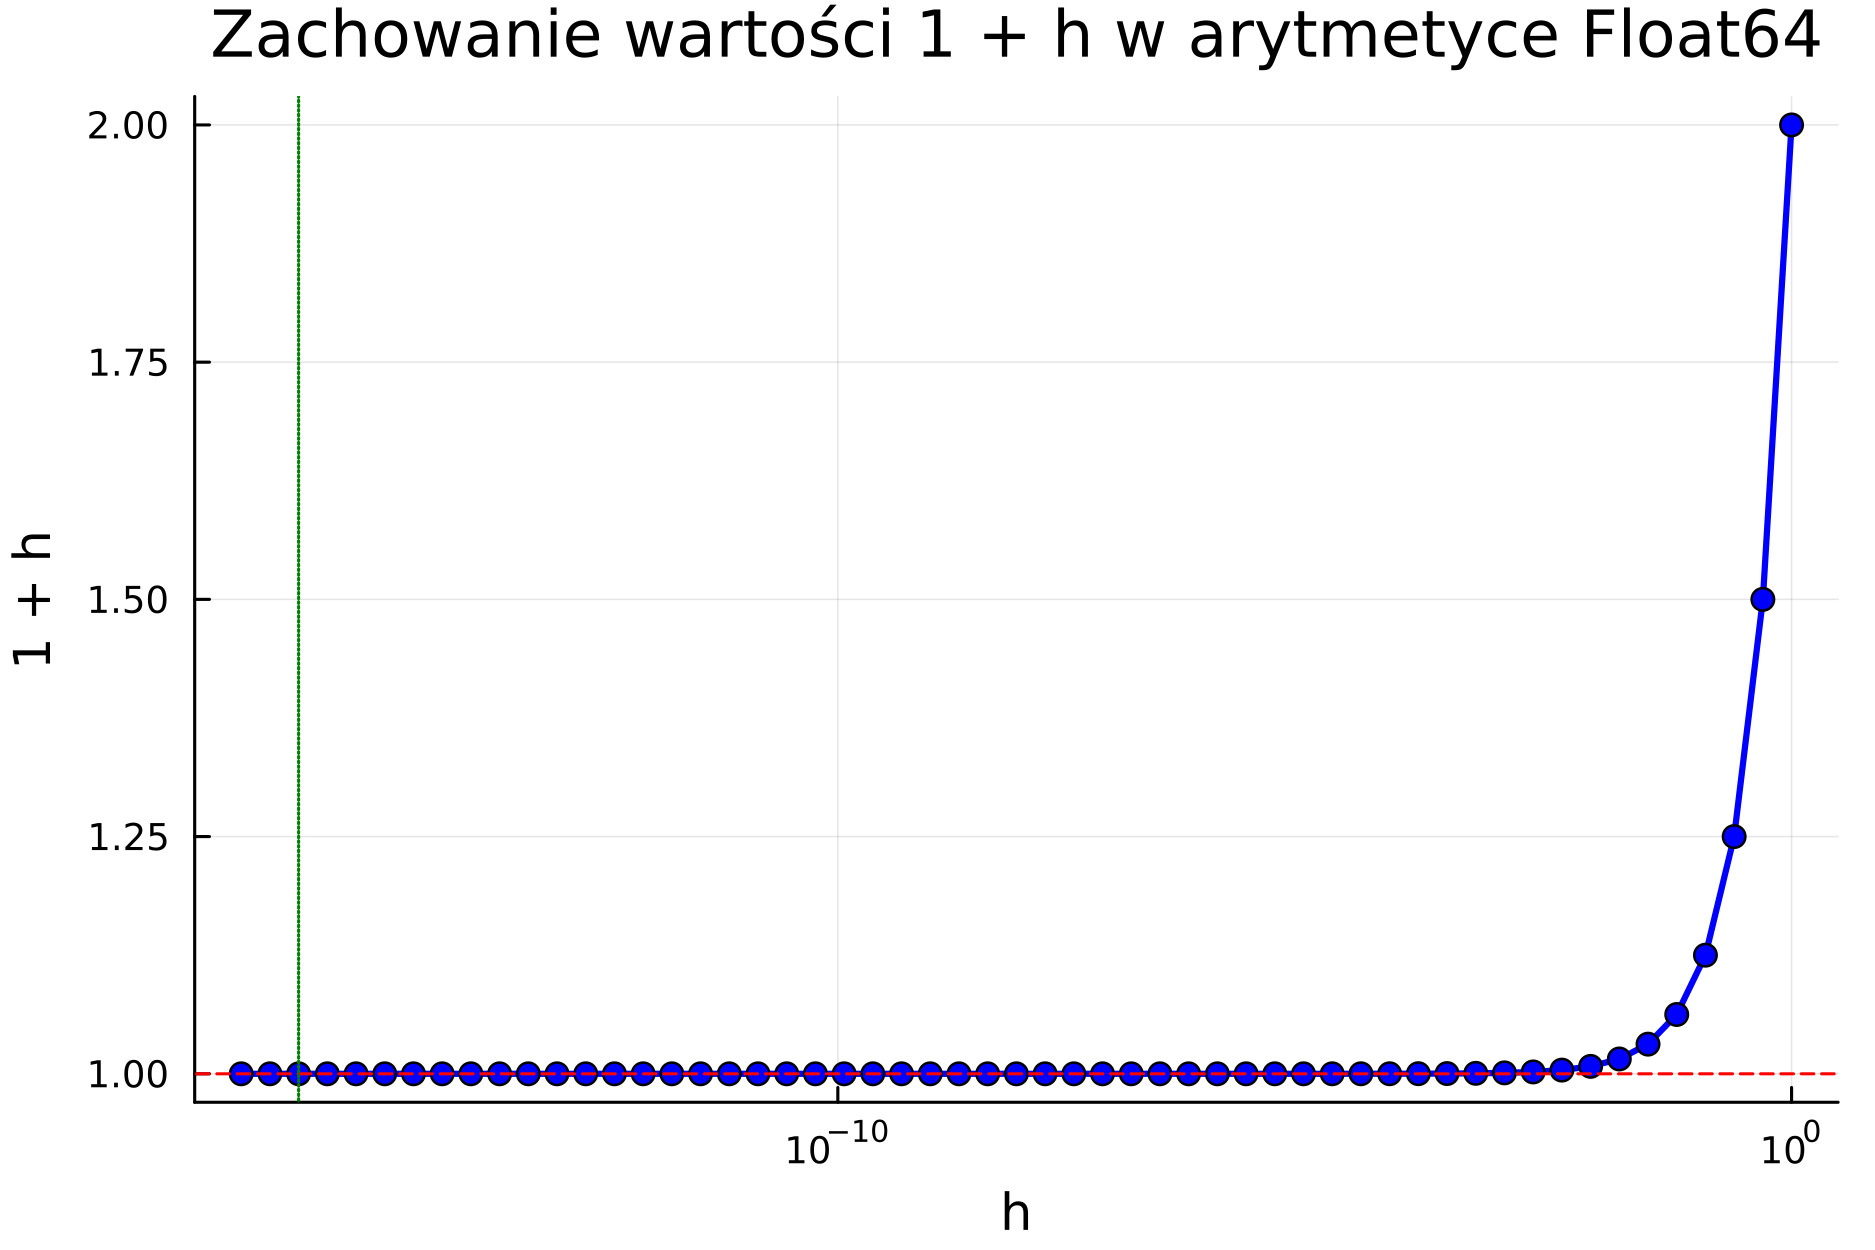
\includegraphics[width=97mm]{plot_2.jpg}
\caption{Wartość 1 + h}
\end{figure}
\subsection{Wnioski}
W zadaniu udało się zaobserwować, jak wartość h wpływa na błąd przybliżenia pochodnej. Dla dużych wartości h błąd jest duży, ponieważ przybliżenie jest niedokładne. Wraz ze zmniejsaniem się h, błąd maleje, aż do pewnego momentu, gdzie zaczyna rosnąć ponownie. Dzieje się tak, ponieważ dla bardzo małych wartości h, różnica $f(x_{0}+h)-f(x_{0})$ staje się bardzo mała i prowadzi do redukcji cyfr znaczących. Dodatkowo, na drugim wykresie widać, że dla bardzo małych wartości h, wartość $1 + h$ jest równa 1, co również wskazuje na utratę precyzji.
\end{document}